It is well known that using $f+1$ replicas can tolerate $f$ crash failures and $2f+1$ can tolerate $f$ silent failures. Actually, it is not difficult to derive that $f_1 + 2f_2 + 1$ replicas can tolerate both crash and silent failures, assuming there are at most $f_1$ crash failure(s) and $f_2$ silent failure(s). We argue that the two schemes presented in Section~\ref{sec:crash_collocation} and~\ref{sec:silent_cp_leap} can be combined to tolerate both types of failures simultaneously, while reducing energy consumption under certain constraints. 


This section presents a case study that tolerates 1 crash failure and 1 silent failure, by using 4 replicas, which is the minimum number of replicas required. The execution dynamics are shown in Figure~\ref{fig:com_failure_model}. 
Two fast replicas will consume data from one end, and the two slow replica will proceed from the opposite end. Voting is invoked periodically to detect silent failure. If neither crash nor silent failure occurs, the four replicas will meet at a rendezvous point, determined by their relative execution rates (Figure~\ref{fig:com1}. 

\begin{figure}[!t]
	\begin{center}
		\subfigure[Non-faulty task.]
		{
			\label{fig:com1}
			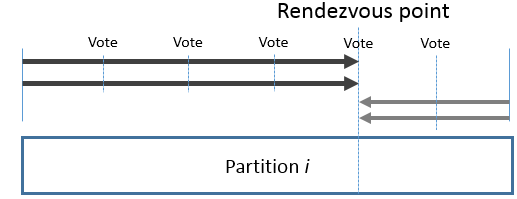
\includegraphics[width=0.9\columnwidth]{figures/combine1}
		}
		\subfigure[Task with a silent failure.]
		{
			\label{fig:com3}
			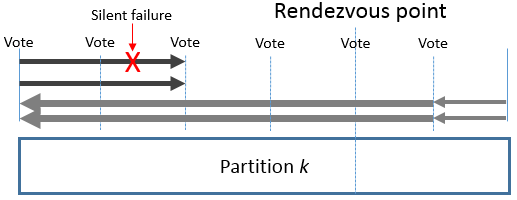
\includegraphics[width=0.9\columnwidth]{figures/combine3}
		}
        \subfigure[Task with a crash failure.]
		{
			\label{fig:com2}
			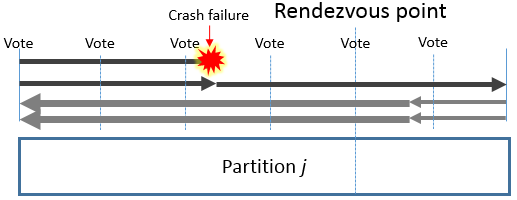
\includegraphics[width=0.9\columnwidth]{figures/combine2}
		}
	\end{center}
	\caption{Illustration of the tolerance of 1 crash failure and 1 silent failure simultaneously.}
	\label{fig:com_failure_model}
\end{figure}

If a failure occurs, there are two execution strategies, based on the type of the failure. If it is a silent failure, let's say a fast replica fails, then both fast replicas can be terminated when they reach an disagreement at the next voting point. In this case, however, the two slow replicas need to proceed beyond the original rendezvous point and process the whole partition, potentially at a higher rate to meet deadline, if any. With two remaining replicas, the system is still able to tolerate a crash failure. The illustration is shown in Figure~\ref{fig:com3}.

If the first failure occurred is a crash failure, a different execution strategy will be applied, as shown in Figure~\ref{fig:com2}. After a crash failure happens, all three remaining replicas need to continue execution and process the whole partition. This allows the system to detect and correct a subsequent silent failure. Similarly, the remaining replicas may speed up after the failure for response time consideration. 